% \newpage

% \section{Расширенное техническое задание}

% В данном разделе представлено техническое задание на разработку системы.


% \subsection{Основание для разработки}

% Программа разрабатывается на основе учебного плана кафедры “Электронные вычислительные машины” по направлению 09.03.01.

% \subsection{Цель и задача}

% Название темы: «Разработка системы оценки и прогнозирования интересов клиентов автостоянки».

% Целью дипломного проекта является автоматизация процесса сбора данных об интересах посетителей парковки и их прогнозирования.

% Задача – проектирование и разработка системы для сбора информации об интересах и их прогнозирования на базе искусственной нейронной сети.


% \subsection{Наименование и область применения}

% Наименование разрабатываемого программного обеспечения: система оценки и прогнозирования интересов клиентов автостоянки. 

% Область применения: прогнозирование интересов посетителей парковки для улучшения сервиса.


% \subsection{Требования к функциональности}

% Программа должна обеспечивать возможность выполнения следующих функций:

% \begin{itemize}
% 	\item определять регистрационный номер автомобиля;
% 	\item определять модель автомобиля
% 	\item анализировать бланки опросов определенного формата;
% 	\item формирование набора данных в файл типа CSV;
% 	\item обучение нейронной сети по сформированному датасету;
% 	\item предсказывать интересы посетителей с использование обученной модели.
% \end{itemize}


% \subsection{Требования к нейронной сети}

% Нейронная сеть должна быть реализована на базе языка программирования Python с использованием библиотеки Tensorflow, Keras.


% \subsection{Требования к бланку}

% Бланк должен содержать вопросы и варианты ответа на вопросы (ДА/НЕТ), а также поле для ввода возраста. Пример представлен на рисунке~\ref{f:blank}.

% \begin{figure}[ht]
% 	\centering
% 	\vspace{\toppaddingoffigure}
% 	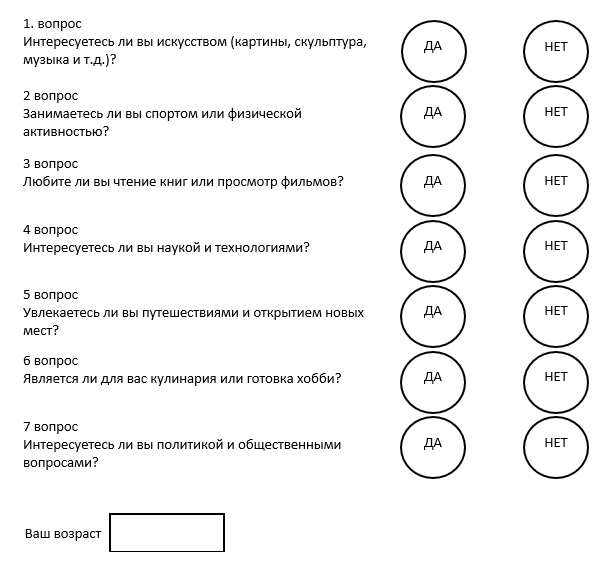
\includegraphics[width=0.7\textwidth]{blank}
% 	\caption{Бланк опроса}
% 	\label{f:blank}
% \end{figure}



% \subsection{Требования к программной документации}

% Состав программной документации должен включать в себя: 

% \begin{itemize}
% 	\item техническое задание; 
% 	\item пояснительная записка, содержащая описание разработки;
% 	\item руководство пользователя.
% \end{itemize}

% Разрабатываемые программные модули должны быть самодокументированы, т.е. тексты программ должны содержать все необходимые комментарии.

% \subsection{Технико-экономические характеристики}

% Реализованное программное обеспечение использует бесплатную модель распространения и разрабатывается с помощью бесплатных решений.


% \section*{Выводы}

% Составлено техническое задание. Были составлены требования к разрабатываемой системе, а также определены основные функции. 



\subsection{Расширенное техническое задание}

Для нагляного отображения доступного пользователю функционала используются диаграмма вариантов использования, которая изображена на рисунке~\ref{f:diag-precedent1}.

\begin{figure}[h!]
    \centering
    \vspace{\toppaddingoffigure}
    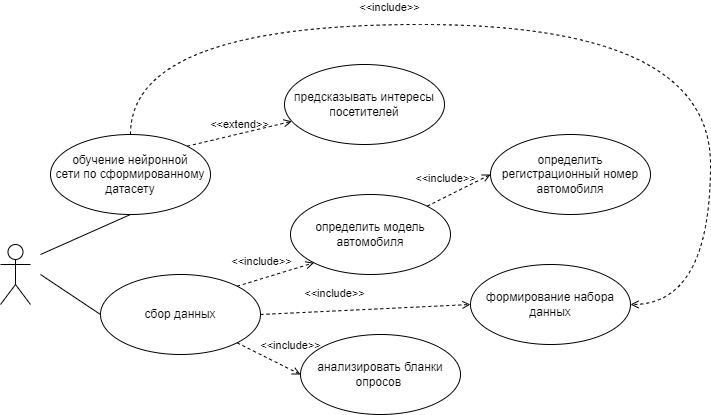
\includegraphics[width=0.7\textwidth]{diag-precedent1}
    \caption{Диаграмма вариантов использования}
    \label{f:diag-precedent1}
\end{figure}

\subsubsection{Основание для разработки}

Программа разрабатывается на основе учебного плана кафедры “Электронные вычислительные машины” по направлению 09.03.01.

\subsubsection{Цель и задача}

Название темы: «Разработка системы оценки и прогнозирования интересов клиентов автостоянки».

Объект - маркетинговое исследование для улучшения качества обслуживания клиентов.

% система оценки и прогнозирования интересов клиентов автостоянки.

Предмет - прогнозирования интересов клиентов автостоянки.

Целью дипломного проекта является помощь маркетологам в понимании предпочтений владельцев автомобилей через автоматизированный сбор и анализ данных, что позволит разрабатывать более точные и персонализированные маркетинговые стратегии. 

Задачи:
\begin{itemize}
    \item автоматизация процесса сбора данных;
    \item распознавание интересов посетителей парковки;
    \item прогнозирование интересов посетителей парковки;
\end{itemize}
% автоматизация процесса сбора данных об интересах посетителей парковки и их прогнозирования.

Результат - разработанная программная система для сбора информации о интересах клиентов и их прогнозироваения. 

\subsubsection{Наименование и область применения}

Наименование разрабатываемого программного обеспечения: система оценки и прогнозирования интересов клиентов автостоянки. 

Область применения: прогнозирование интересов посетителей парковки для улучшения сервиса.


\subsubsection{Требования к функциональности}

Программа должна обеспечивать возможность выполнения следующих функций:

\begin{itemize}
	\item определять регистрационный номер автомобиля;
	\item определять модель автомобиля
	\item анализировать бланки опросов определенного формата;
	\item формирование набора данных в файл типа CSV;
	\item обучение нейронной сети по сформированному датасету;
	\item предсказывать интересы посетителей с использование обученной модели.
\end{itemize}


\subsubsection{Требования к нейронной сети}

Нейронная сеть должна быть реализована на базе языка программирования Python с использованием библиотеки Tensorflow, Keras.


\subsubsection{Требования к бланку}

Бланк должен содержать вопросы и варианты ответа на вопросы (ДА/НЕТ), а также поле для ввода возраста. Пример представлен на рисунке~\ref{f:blank}.

\begin{figure}[ht]
	\centering
	\vspace{\toppaddingoffigure}
	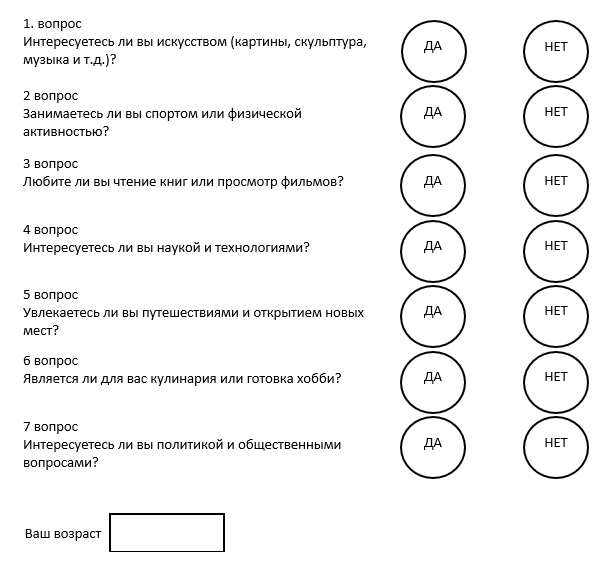
\includegraphics[width=0.7\textwidth]{blank}
	\caption{Бланк опроса}
	\label{f:blank}
\end{figure}



\subsubsection{Требования к программной документации}

Состав программной документации должен включать в себя: 

\begin{itemize}
	\item техническое задание; 
	\item пояснительная записка, содержащая описание разработки;
	\item руководство пользователя.
\end{itemize}

Разрабатываемые программные модули должны быть самодокументированы, т.е. тексты программ должны содержать все необходимые комментарии.

\subsubsection{Технико-экономические характеристики}

Реализованное программное обеспечение использует бесплатную модель распространения и разрабатывается с помощью бесплатных решений.